\documentclass{report}
\usepackage{listings}
\usepackage{graphicx}

\begin{document}
\title{Report 3 - CUDA}
\begin{figure}
    \centering
    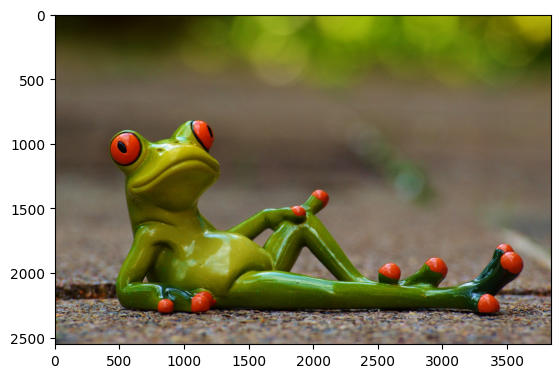
\includegraphics[width=1\linewidth]{base_frog_2D.png}
\end{figure}
\maketitle


\section{2D Grayscaling}
\begin{lstlisting}[language=Python]
@cuda.jit
def grayscale2D(src, dst):
  # where are we in the input?
  x = cuda.threadIdx.x + cuda.blockIdx.x * cuda.blockDim.x
  y = cuda.threadIdx.y + cuda.blockIdx.y * cuda.blockDim.y
  if y < src.shape[0] and x < src.shape[1]:
    g = np.uint8((src[y, x, 0] + src[y, x, 1] + src[y, x, 2]) / 3)
    dst[y, x, 0] = dst[y, x, 1] = dst[y, x, 2] = g

devSrc2 = cuda.to_device(img)
devDst2 = cuda.device_array_like(img)

#single blank kernel call with arbitrary gridSide 8
blankGridSize2 = ((width+8-1)//8,(height+8-1)//8)
grayscale2D[blankGridSize2, (8,8)](devSrc2, devDst2)

times = []
range_avg = 5
blockSides = range(1,33)
for blockSide in blockSides:
  avg = 0
  for i in range(range_avg):
    blockSize2 = (blockSide, blockSide)

    #rounding up
    gridSideX = (width+blockSide-1)//blockSide
    gridSideY = (height+blockSide-1)//blockSide
    gridSize2 = (gridSideX,gridSideY)

    start=time.time()
    
    #kernel call
    grayscale2D[gridSize2, blockSize2](devSrc2, devDst2)

    cuda.synchronize()
    stop=time.time()
    avg+=stop-start
  avg/=range_avg
  times.append(avg)
\end{lstlisting}


\begin{itemize}
    \item \textbf{2D best blockside: 8 with duration:  0.0010}
    \item vs.
    \item \textbf{1D best blockside: 128 with duration: duration 0.0046}
\end{itemize}
\begin{figure}
    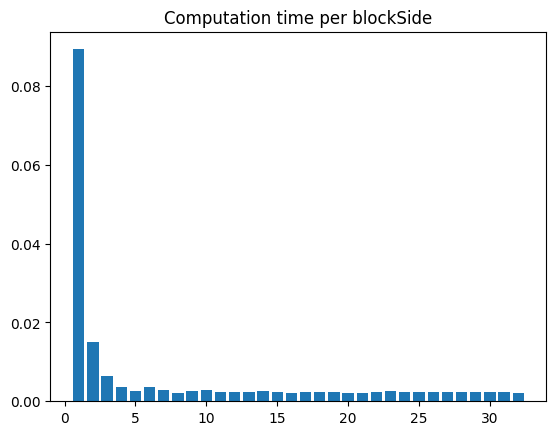
\includegraphics[width=0.5\linewidth]{2D_speedup_barplot.png}
    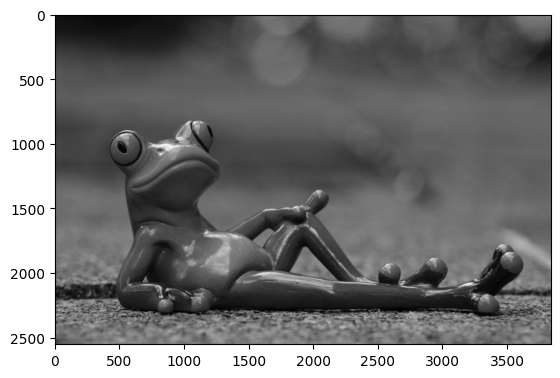
\includegraphics[width=0.5\linewidth]{frog_2D.png}
\end{figure}


\section{Exercise1}
\begin{itemize}
    \item Hardware limit of 512 threads/block means 32x32=1024 doesn't fit as a block size.
    \item Maximizing SM: both 8x8 and 16x16 use all blocks of SM (%SM_max_size=0)
    \item However 8x8 blocks would mean 16 blocks/SM which doesn't fit the 8 blocks/SM limit. 16x16 is 4 which is fine.
    \item In the end only \textbf{16x16} fits. 32 threads/warp would mean there would be 8warps/block.
\end{itemize}


\section{Exercise2}
\begin{itemize}
    \item 4*128=512
    \item 4*256=1024
    \item \textbf{3*512=1536 this is the best config}
    \item 1*1024=1024
\end{itemize}


\section{Exercise3}
\begin{itemize}
    \item (2000+512-1)//512 = 4
    \item There will be 4 blocks of 512 threads, meaning \textbf{2048} threads in the grid.
\end{itemize}
\end{document}